\documentclass[conference]{IEEEtran}
\usepackage{cite}
\usepackage{amsmath,amssymb,amsfonts}
\usepackage{graphicx}
\usepackage{booktabs}
\usepackage{array}
\graphicspath{{figures/}}

\begin{document}

\title{StereoLite: Real-Time Zero-Shot Stereo Matching on Embedded Hardware}

\author{\IEEEauthorblockN{Nazib Abrar, Md Raihanul Haque Rahi, Md Zunaid Hossen}
\IEEEauthorblockA{Department of Mechatronics Engineering\\
Rajshahi University of Engineering \& Technology\\
Rajshahi, Bangladesh}}

\maketitle

\begin{abstract}
Dense depth from a stereo pair must be produced in real time on embedded accelerators for mobile robots, drones, and augmented reality rigs. However, the networks that generalize across domains are large iterative or foundation-scale models, while compact networks tend to collapse once the test domain departs from their training data. We present StereoLite, a 2.96 M parameter stereo network that composes known efficient mechanisms at an edge budget: a slanted tile-plane state, initialized from a single coarse group-wise cost volume and refined by a convolutional GRU over eight updates across three scales, is corrected by a narrow-band geometry encoding volume through a learned fail-soft gate. Trained only on SceneFlow, a single checkpoint evaluated under one fixed protocol attains 4.33, 3.93, 3.96, and 10.9 percent D1-all on the KITTI 2012, KITTI 2015, ETH3D, and Middlebury 2014 training sets without fine-tuning, alongside 0.78 px end-point error on the FlyingThings3D test set. A six-change graph optimization and INT8 TensorRT export run the model at 36.3 ms per frame (27.5 FPS) on a Jetson Orin Nano within roughly 0.15 GB of memory, and accuracy degrades gracefully under up to one pixel of vertical rectification error. These are training-split evaluations under our own protocol rather than official leaderboard submissions.
\end{abstract}

\begin{IEEEkeywords}
stereo matching, disparity estimation, edge deployment, zero-shot generalization, recurrent refinement
\end{IEEEkeywords}

\section{Introduction}
\label{sec:intro}
Stereo matching estimates a dense disparity map from a rectified image pair, from which metric depth follows as $Z = fB/d$ for focal length $f$ and baseline $B$. Because it recovers metric structure from two passive cameras, it is a natural depth source for platforms that cannot carry LiDAR or afford active sensing: mobile robots, drones, and embedded vision rigs. On such platforms the depth estimator must share an edge accelerator with the rest of the software stack, which imposes hard limits on parameters, latency, and memory.

Deep stereo networks have moved far past classical pipelines \cite{scharstein2002taxonomy,hirschmuller2008sgm,zbontar2016mccnn} in accuracy, first through 3D cost-volume regularization \cite{kendall2017gcnet,chang2018psmnet,guo2019gwcnet,zhang2019ganet} and then through iterative recurrent refinement \cite{lipson2021raftstereo,li2022crestereo,xu2023igev,wang2024selective}. However, the models that transfer best to unseen domains are the largest ones: foundation-scale networks such as FoundationStereo \cite{wen2025foundationstereo} reach remarkable zero-shot accuracy with hundreds of millions of parameters, and even the strong iterative baselines run hundreds of milliseconds per frame on desktop GPUs. Efficient networks \cite{khamis2018stereonet,wang2019anynet,tonioni2019madnet,duggal2019deeppruner,xu2021bgnet,bangunharcana2021coex,tankovich2021hitnet,shamsafar2022mobilestereonet,guo2025lightstereo} meet the latency budget but are usually reported only in domain; when they are tested across domains, accuracy often degrades sharply. It is still difficult to obtain usable cross-domain accuracy, real-time embedded latency, and a quantization-clean operator set in one network.

One major problem with current efficient designs is how to retain the mechanisms that carry generalization once the parameter budget shrinks. HITNet \cite{tankovich2021hitnet} showed that a slanted tile-plane state can replace a dense cost volume at under a million parameters, but its single pass per scale limits refinement. RAFT-Stereo \cite{lipson2021raftstereo} showed that a recurrent update operator concentrates capacity efficiently, but its all-pairs correlation and many-iteration schedule target desktop budgets. IGEV-Stereo \cite{xu2023igev} showed that a geometry encoding volume warm-starts the iterations, at the cost of a full-range 3D volume. Each mechanism is established; what the literature does not report is whether their combination, cut down to an embedded budget, preserves enough cross-domain accuracy to be useful in the field.

In this work, we present StereoLite, a 2.96 M parameter stereo network that composes these mechanisms under an explicit edge envelope. A truncated detection backbone and a separate left-image context encoder feed a group-wise cost volume \cite{guo2019gwcnet} at 1/16 resolution, which seeds a slanted tile-plane state in the manner of HITNet \cite{tankovich2021hitnet}. A convolutional GRU \cite{lipson2021raftstereo} refines the state with CREStereo-style local correlation \cite{li2022crestereo} over eight updates across three scales, with plane-aware propagation between scales. A narrow-band geometry encoding volume, in the spirit of IGEV-Stereo \cite{xu2023igev}, contributes an independent proposal that a learned fail-soft gate blends in only where it helps. We claim no novel block; the contribution is the composition, the edge-side engineering, and the measurement:
\begin{itemize}
\item We assemble tile-plane state, recurrent refinement, local correlation, and a narrow-band geometry volume with learned fail-soft fusion into a 2.96 M parameter network whose every operator quantizes to INT8.
\item We report a zero-shot quartet from one SceneFlow-trained checkpoint under one protocol: 4.33, 3.93, 3.96, and 10.9 percent D1-all on KITTI 2012, KITTI 2015, ETH3D, and Middlebury 2014, with 0.78 px end-point error in domain.
\item We deploy the network on a Jetson Orin Nano at 36.3 ms per frame (27.5 FPS) via a six-change graph optimization (1.74$\times$ speedup at full precision) and a calibrated INT8 TensorRT engine.
\item We characterize robustness to imperfect rectification, both under controlled vertical offsets and on 997 pairs from a physical 52 mm baseline rig, where the model agrees with a FoundationStereo reference to 1.45 px mean end-point error.
\end{itemize}

\section{Related Work}
\label{sec:related}

\subsection{Efficient Stereo Networks}
StereoNet \cite{khamis2018stereonet} established the coarse-volume-plus-refinement template for real-time stereo, and AnyNet \cite{wang2019anynet} made the accuracy-latency trade-off adjustable at inference time. MADNet \cite{tonioni2019madnet} paired a compact pyramid network with online adaptation, and DeepPruner \cite{duggal2019deeppruner} pruned the disparity search space with differentiable PatchMatch. BGNet \cite{xu2021bgnet} upsampled a low-resolution cost volume through a learned bilateral grid, and CoEx \cite{bangunharcana2021coex} excited cost-volume channels with image guidance. MobileStereoNet \cite{shamsafar2022mobilestereonet} transferred mobile-friendly convolutions to both 2D and 3D stereo networks, LightStereo \cite{guo2025lightstereo} boosted channel-wise 2D aggregation, and BANet \cite{xu2025banet} split aggregation into detail and smoothness branches for mobile GPUs. These networks meet embedded budgets, but their published results are dominated by in-domain benchmarks; cross-domain accuracy at the edge budget is far less documented.

\subsection{Iterative Refinement}
RAFT-Stereo \cite{lipson2021raftstereo} recast stereo as recurrent refinement of a disparity field by a convolutional GRU that indexes a precomputed correlation pyramid, with a separate context encoder conditioning the update. CREStereo \cite{li2022crestereo} replaced all-pairs correlation with an adaptive local search, which also confers tolerance to imperfect rectification. IGEV-Stereo \cite{xu2023igev} warm-started the recurrence from a regularized geometry encoding volume, cutting the iterations needed, and Selective-Stereo \cite{wang2024selective} routed frequency-specific information through parallel GRU branches. Pip-Stereo \cite{zheng2026pipstereo} prunes iterations progressively for efficiency. StereoLite borrows the recurrent operator and the warm-start idea but runs only eight updates at coarse scales, on a tile-plane state rather than a dense field.

\subsection{Tile and Plane Representations}
HITNet \cite{tankovich2021hitnet} represents disparity as a grid of slanted tiles, each carrying a disparity, two plane slopes, and a descriptor, and propagates these hypotheses coarse to fine without a dense cost volume; the result is real-time accuracy at under a million parameters. StereoLite keeps this state representation and its plane-aware cross-scale propagation, but replaces the single pass per scale with iterated GRU updates, a change our ablations show is load bearing.

\subsection{Zero-Shot Generalization}
DSMNet \cite{zhang2020dsmnet} introduced domain-invariant normalization for synthetic-to-real transfer, and HVT \cite{chang2023hvt} generalized through hierarchical visual transformations of the training data. The recent foundation-model era attacks the same problem with scale: FoundationStereo \cite{wen2025foundationstereo} trains on a million-pair corpus with a rich monocular prior, DEFOM-Stereo \cite{jiang2025defom} and MonSter \cite{cheng2025monster} integrate monocular depth foundation models, and Stereo Anywhere \cite{bartolomei2025stereoanywhere} fuses stereo and monocular cues for robustness. LiteAnyStereo \cite{jing2025liteanystereo} shows that a non-iterative 7.6 M network can inherit much of this robustness through a three-stage knowledge distillation pipeline. These results frame our question from the opposite side: how much zero-shot accuracy survives at 2.96 M parameters with supervised SceneFlow training alone.

\section{Method}
\label{sec:method}

\subsection{Overview}
Figure \ref{fig:arch} shows the pipeline. StereoLite is a coarse-to-fine tile-hypothesis network with light recurrent refinement. A shared encoder extracts matching features from both views and a separate context encoder processes the left image; a group-wise cost volume at 1/16 resolution initializes a slanted tile state; a convolutional GRU refines the state over two iterations at 1/16, three at 1/8, and three at 1/4 resolution, with plane-aware propagation between scales; a narrow-band geometry encoding volume at 1/4 resolution corrects the estimate through a learned fail-soft gate; and plane rendering with two learned convex upsampling stages recovers the full-resolution disparity. The full network holds 2.9631 M trainable parameters.

\begin{figure*}[!htbp]
\centering
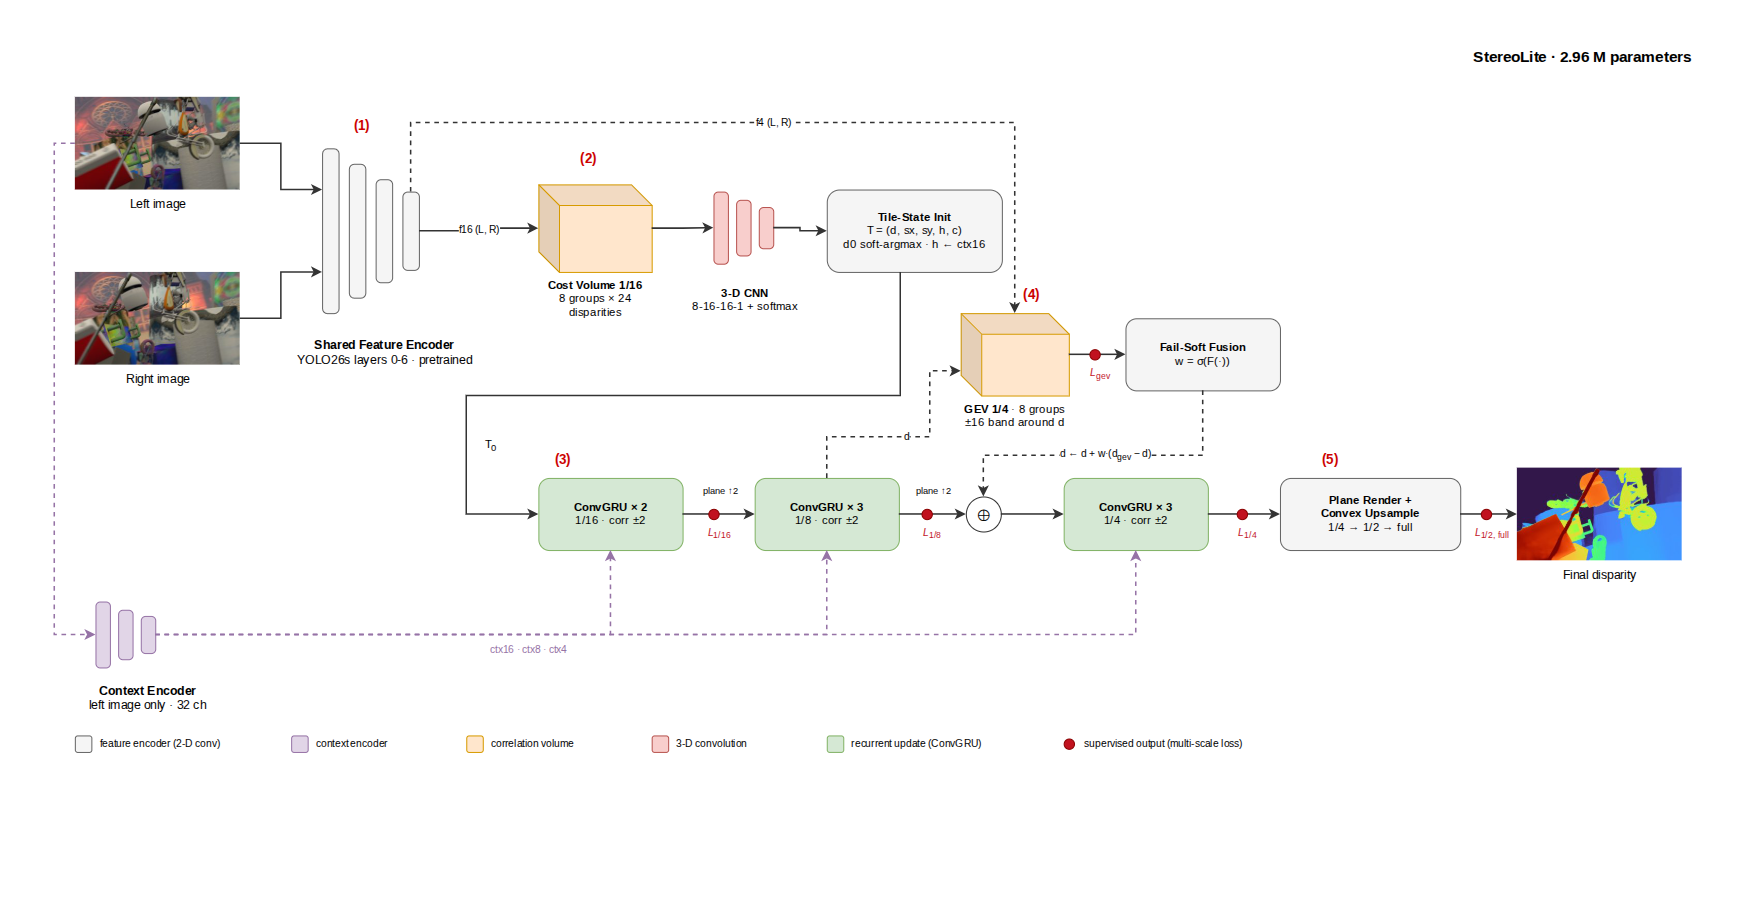
\includegraphics[width=\textwidth]{fig_3_1_architecture_preview}
\caption{\textbf{StereoLite architecture overview.} A shared truncated YOLO26s encoder and a separate left-image context encoder feed a 1/16-resolution group-wise cost volume that initializes a slanted tile state; a ConvGRU refines the state over eight updates across three scales with plane-aware propagation, a narrow-band geometry encoding volume is fused at 1/4 resolution through a learned fail-soft gate, and plane rendering with two learned convex upsampling stages produces the full-resolution disparity.}
\label{fig:arch}
\end{figure*}

\subsection{Feature and Context Encoders}
The matching encoder is a YOLO26s backbone truncated after its first seven blocks, producing features at 1/4, 1/8, and 1/16 resolution with 128, 256, and 256 channels. Detection features are pretrained to localize objects across scales, which is close to what matching requires, and in our encoder ablation this backbone beat both a hand-built GhostConv stack and its smaller YOLO26n sibling on every accuracy metric at a 2 ms latency cost. The two views are concatenated along the batch dimension and pass through a single shared invocation. A separate context encoder processes the left image alone and projects it to a 32-channel quarter-resolution context map, pooled to the coarser scales. Matching evidence and recurrent context are kept in separate streams: if the matching features also served as context, the recurrent unit could not separate appearance from correspondence, and the RAFT-Stereo lineage \cite{lipson2021raftstereo} established that a dedicated context path improves refinement.

\subsection{Cost-Volume Initialization}
Tile initialization builds a group-wise correlation volume \cite{guo2019gwcnet} at 1/16 resolution. For each of $G=8$ feature groups and each integer disparity hypothesis, the matching score is
\begin{equation}
C(g,d,y,x) = \frac{1}{C/G}\sum_{c=1}^{C/G}
  f_{L}^{\,g,c}(y,x)\, f_{R}^{\,g,c}(y,\,x-d),
\label{eq:gwc}
\end{equation}
where $f_{L}^{\,g,c}$ and $f_{R}^{\,g,c}$ are the $c$-th channel of group $g$ of the left and right feature maps and $d \in \{0,\dots,23\}$ indexes 24 hypotheses, spanning roughly 0 to 368 full-resolution pixels. A small 3D CNN with an 8-16-16-1 channel schedule regularizes the volume, and a softmax along the disparity axis yields a distribution $p(d)$ from which the soft-argmin \cite{kendall2017gcnet} reads the initial state,
\begin{equation}
d_{0} = \sum_{d} p(d)\, d, \qquad
c_{0} = \max_{d}\, p(d),
\label{eq:init}
\end{equation}
where $d_0$ is the expected disparity and $c_0$ a confidence. Plane slopes start at zero and the hidden state starts from the coarsest context map. Restricting the volume to a single coarse scale keeps the peak activation memory inside the edge envelope.

\subsection{Recurrent Tile Refinement}
Separate refinement modules operate at 1/16, 1/8, and 1/4 resolution; weights are not shared because the feature channel counts differ. At each iteration the right features are warped by the current disparity, and a differentiable local correlation in the manner of CREStereo \cite{li2022crestereo} is evaluated over five offsets within $\pm 2$ px. The recurrent input assembles
\begin{equation}
x = \bigl[\, f_{L},\ \mathcal{W}(f_{R};d),\ d,\ s_{x},\ s_{y},\
  c,\ \mathrm{corr},\ \mathrm{ctx} \,\bigr],
\label{eq:gruinput}
\end{equation}
where $\mathcal{W}(f_{R};d)$ denotes the warped right features, $s_x, s_y$ the plane slopes, $\mathrm{corr}$ the local correlation, and $\mathrm{ctx}$ the scale-matched context. A convolutional GRU \cite{lipson2021raftstereo} with a 32-channel hidden state updates
\begin{equation}
\begin{aligned}
z &= \sigma\!\bigl(\mathrm{Conv}([h,x])\bigr), \quad
r = \sigma\!\bigl(\mathrm{Conv}([h,x])\bigr),\\
q &= \tanh\!\bigl(\mathrm{Conv}([r \odot h,\,x])\bigr), \quad
h' = (1-z) \odot h + z \odot q,
\end{aligned}
\label{eq:gru}
\end{equation}
where $\odot$ is the element-wise product. A two-layer head with 48 hidden channels predicts residuals for disparity, both slopes, and confidence, and a learned gate emits four sigmoid weights that scale each residual; a softplus keeps disparity non-negative. The schedule runs two iterations at 1/16, three at 1/8, and three at 1/4, for eight learned updates in total.

Between scales, propagation carries the tile state to the finer grid along its slanted-surface hypothesis rather than by plain interpolation, following HITNet \cite{tankovich2021hitnet}:
\begin{equation}
d_{\mathrm{child}} = 2\,\mathcal{B}(d_{\mathrm{parent}})
  + 2\,s_{x}\,\Delta x + 2\,s_{y}\,\Delta y,
\label{eq:prop}
\end{equation}
where $\mathcal{B}$ is bilinear resampling, $\Delta x, \Delta y \in \{-0.25, +0.25\}$ are the child offsets, and the factor of two rescales disparity to the finer grid. Sub-pixel structure is retained without rebuilding a cost volume at any finer level.

\subsection{Narrow-Band Geometry Volume and Fail-Soft Fusion}
A geometry encoding volume in the spirit of IGEV-Stereo \cite{xu2023igev} adds an independent proposal at 1/4 resolution. Rather than spanning the full disparity range, it samples 33 hypotheses in a band of $\pm 16$ around the current tile disparity; since the coarse initialization has already localized the disparity, the band's job is correction, not search, and our efficiency ablation validates the narrowing as accuracy neutral while removing roughly a quarter of the model's multiply-accumulate operations. The volume is regularized by three 3D convolutions with 16 hidden channels, and its softmax distribution yields an expected disparity $d_{\mathrm{gev}}$, a confidence $c_{\mathrm{gev}}$, and a projected geometry feature $g_{\mathrm{gev}}$. The proposal is not substituted unconditionally. A learned gate produces a scalar blend weight,
\begin{equation}
\begin{aligned}
w &= \sigma\!\Bigl(F\bigl([\mathrm{ctx}_{4},\, g_{\mathrm{gev}},\, c,\,
  c_{\mathrm{gev}},\, \lvert d_{\mathrm{gev}} - d \rvert,\, d]\bigr)\Bigr),\\
d_{\mathrm{fused}} &= \mathrm{softplus}\bigl(d + w\,(d_{\mathrm{gev}} - d)\bigr),
\end{aligned}
\label{eq:failsoft}
\end{equation}
where $F$ is the fusion network. We initialize the final-layer bias of $F$ to $-4$, so the initial weight is approximately 0.018 and training begins close to the stable recurrent baseline; the network then learns where the geometry proposal helps. This fail-soft design stops the global branch from corrupting regions the recurrent path already resolves well.

\subsection{Plane Rendering and Convex Upsampling}
Before upsampling, a plane-rendering step reconstructs each tile from its disparity and slopes and applies an edge gate; in our boundary-sharpness ablation this step cut the bad-0.5 rate from 55.36 to 42.91 percent. The rendered 1/4 disparity is then upsampled to full resolution in two learned $2\times$ stages, each predicting a softmax over the $3\times 3$ coarse neighborhood of every output subpixel, so the upsampled disparity is a convex combination of nearby coarse values, as in RAFT-Stereo \cite{lipson2021raftstereo}.

\subsection{Training Objective}
The network trains under an eleven-term multi-scale objective. A pixel is valid when its ground-truth disparity is finite and lies between 0 and 320 px; lower-scale predictions are resized to full resolution and rescaled before comparison. The objective is
\begin{equation}
\begin{aligned}
\mathcal{L} ={}& 1.0\,\mathcal{L}_{1}(d_{\mathrm{full}})
 + 0.5\,\mathcal{L}_{1}(d_{1/2})
 + 0.3\,\mathcal{L}_{1}(d_{1/4})\\
&+ 0.2\,\mathcal{L}_{1}(d_{1/8})
 + 0.1\,\mathcal{L}_{1}(d_{1/16})
 + 0.15\,\mathcal{L}_{1}(d_{\mathrm{gev}})\\
&+ 0.5\,\mathcal{L}_{\mathrm{grad}}
 + 0.2\,\mathcal{L}_{\mathrm{thr}}
 + 0.2\,\mathcal{L}_{\mathrm{D1}}\\
&+ 0.02\,\mathcal{L}_{\mathrm{smooth}}
 + 0.3\,\mathcal{L}_{\mathrm{slant}},
\end{aligned}
\label{eq:loss}
\end{equation}
where $\mathcal{L}_1$ is the masked mean absolute disparity error, $\mathcal{L}_{\mathrm{grad}}$ a Sobel gradient-consistency term, $\mathcal{L}_{\mathrm{thr}}$ a hinge stacked over the error thresholds $\{0.5, 1, 2, 3\}$ px, $\mathcal{L}_{\mathrm{D1}}$ a D1-relative hinge \cite{menze2015kitti}, $\mathcal{L}_{\mathrm{smooth}}$ an edge-aware smoothness term, and $\mathcal{L}_{\mathrm{slant}}$ a gated slant-supervision term that trains the plane slopes only where they are trustworthy. This composition was chosen by ablation: across nine formulations, the threshold stack combined with the D1 hinge was the only one to win end-point error and the outlier rates together.

\subsection{Training Protocol}
We train on the full SceneFlow finalpass corpus \cite{mayer2016sceneflow}, 35{,}454 pairs, for 60{,}000 steps at batch 32 in bfloat16 mixed precision on a single A100 80 GB GPU, using AdamW with weight decay $10^{-5}$ and a OneCycle schedule peaking at $8\times 10^{-4}$. Training samples random $384\times 640$ co-located crops from the native $960\times 540$ frames, which preserves native disparity magnitudes; our input-protocol ablation shows this native-crop protocol substantially outperforms downscaling the frame before cropping. Three augmentations apply: asymmetric color jitter, right-image-only random erasing, and random scaling. The best checkpoint, selected on a fixed validation subset, occurs at step 53{,}000.

\section{Experiments}
\label{sec:exp}

\subsection{Setup}
We report end-point error (EPE), root-mean-square error, median absolute error, the bad-$t$ rates for $t \in \{0.5,1,2,3\}$ px, and D1-all \cite{menze2015kitti}, averaged per image over valid pixels. In-domain evaluation uses the full FlyingThings3D test set \cite{mayer2016sceneflow}, 4{,}370 pairs at native $960\times 540$ resolution. Zero-shot evaluation applies one fixed protocol to every dataset: images are resized to $384\times 640$, ground truth is scaled by $s_x = 640/W$, pixels that are invalid or exceed 192 px after resizing are masked, and metrics are computed over valid pixels. All zero-shot numbers are computed on the public training splits of KITTI 2012 \cite{geiger2012kitti}, KITTI 2015 \cite{menze2015kitti}, ETH3D \cite{schops2017eth3d}, and Middlebury 2014 \cite{scharstein2014middlebury} under our own protocol; they are not official leaderboard submissions, and we label them accordingly. Latency is measured at batch 1 and $384\times 640$ with 10 warm-up and 100 timed passes.

\subsection{In-Domain Accuracy}
Table \ref{tab:indomain} reports the full FlyingThings3D test-set result. The model reaches 0.781 px EPE and 3.40 percent D1-all. The metric spread is informative: the median of 0.130 px is six times smaller than the mean, and the RMSE of 3.64 is nearly five times larger, so most pixels are highly accurate while a small population of large outliers sets the average. Errors above half a pixel affect 15.32 percent of pixels but above three pixels only 4.00 percent; failures concentrate at occlusion boundaries and thin structures, consistent with recurrent reasoning at quarter resolution and an upsampler that recombines disparity but cannot invent it. Figure \ref{fig:curves} shows the training trajectory: validation EPE bottoms out near step 53{,}000 and holds flat thereafter, so we take the best checkpoint there.

\begin{table}[!htbp]
\centering
\caption{\textbf{In-domain accuracy on the full FlyingThings3D test set} (4{,}370 pairs, native $960\times 540$).}
\label{tab:indomain}
\footnotesize
\setlength{\tabcolsep}{3.6pt}
\begin{tabular}{cccccccc}
\toprule
EPE & RMSE & Med. & bad-0.5 & bad-1 & bad-2 & bad-3 & D1-all\\
(px) & (px) & (px) & (\%) & (\%) & (\%) & (\%) & (\%)\\
\midrule
0.781 & 3.64 & 0.130 & 15.32 & 8.92 & 5.34 & 4.00 & 3.40\\
\bottomrule
\end{tabular}
\end{table}

\begin{figure}[!htbp]
\centering
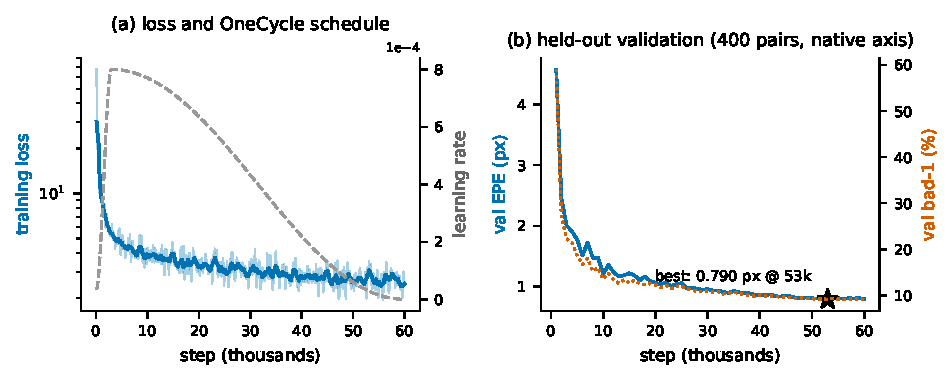
\includegraphics[width=\columnwidth]{fig_4_1_training_curves}
\caption{\textbf{Training loss and validation accuracy over the 60k-step run.} Validation EPE reaches its floor near step 53{,}000, where the reported checkpoint is taken.}
\label{fig:curves}
\end{figure}

\subsection{Zero-Shot Generalization}
Table \ref{tab:zeroshot} is the paper's central result: one checkpoint, trained only on synthetic SceneFlow, evaluated on four real benchmarks under one protocol. On the driving scenes of KITTI 2012 and 2015 the model attains 4.33 and 3.93 percent D1-all at 0.823 px EPE; on the indoor and outdoor scenes of ETH3D it attains 3.96 percent D1-all at 0.930 px. Middlebury 2014, whose high-resolution indoor scenes contain thin repeated structures and disparities near the evaluation cap, is the hardest of the four at 1.71 px EPE and 10.9 percent D1-all. The per-domain spread is narrow outside Middlebury, indicating that the synthetic-to-real gap, not any single domain, sets the operating level.

\begin{table}[!htbp]
\centering
\caption{\textbf{Zero-shot quartet from a single SceneFlow-trained checkpoint.} Evaluation on public training splits under our fixed protocol (resize to $384\times 640$, ground truth scaled by $s_x$, disparities above 192 px masked); not leaderboard submissions.}
\label{tab:zeroshot}
\footnotesize
\setlength{\tabcolsep}{2.6pt}
\begin{tabular}{lccccc}
\toprule
Dataset & Pairs & EPE (px) & bad-1 (\%) & bad-2 (\%) & D1-all (\%)\\
\midrule
KITTI 2012 \cite{geiger2012kitti} & 194 & 0.823 & 16.53 & 6.96 & 4.33\\
KITTI 2015 \cite{menze2015kitti} & 200 & 0.823 & 17.99 & 6.42 & 3.93\\
ETH3D \cite{schops2017eth3d} & 27 & 0.930 & 15.18 & 6.47 & 3.96\\
Middlebury 2014 \cite{scharstein2014middlebury} & 23 & 1.71 & 23.9 & 14.5 & 10.9\\
\bottomrule
\end{tabular}
\end{table}

On Middlebury 2014 we further compare against two public checkpoints re-evaluated under the identical protocol (Table \ref{tab:mb14}). StereoLite is the smallest model in the comparison at 2.96 M parameters and the fastest of the three on device-class hardware after optimization. A gap remains to LiteAnyStereo \cite{jing2025liteanystereo} at 6.9 percent and 16-iteration IGEV-Stereo \cite{xu2023igev} at 5.0 percent D1-all; both are substantially larger, and LiteAnyStereo additionally benefits from a three-stage knowledge distillation pipeline that our supervised-only recipe does not use. Figure \ref{fig:pareto} places the three models on the accuracy-versus-parameters front.

\begin{table}[!htbp]
\centering
\caption{\textbf{Zero-shot Middlebury 2014 comparison} (23 perfect-set scenes; identical protocol for all models; our re-evaluation of public checkpoints; T4 fp32 eager latency).}
\label{tab:mb14}
\footnotesize
\setlength{\tabcolsep}{3.4pt}
\begin{tabular}{lcccc}
\toprule
Model & Params (M) & T4 (ms) & EPE (px) & D1-all (\%)\\
\midrule
StereoLite (ours) & \textbf{2.96} & 86 & 1.71 & 10.9\\
LiteAnyStereo \cite{jing2025liteanystereo} & 7.60 & 64 & 1.17 & 6.9\\
IGEV-Stereo (16 it.) \cite{xu2023igev} & 12.60 & 305 & \textbf{0.86} & \textbf{5.0}\\
\bottomrule
\end{tabular}
\end{table}

\begin{figure}[!htbp]
\centering
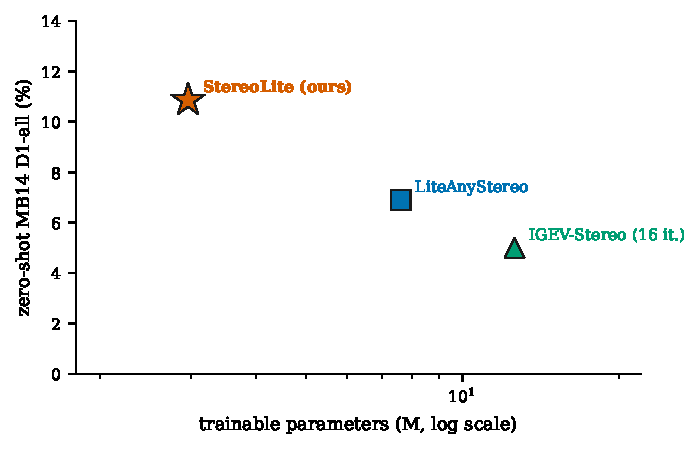
\includegraphics[width=0.9\columnwidth]{fig_4_8_pareto_ours}
\caption{\textbf{Zero-shot Middlebury 2014 D1-all against trainable parameters.} StereoLite occupies the low-parameter end of the front below the larger distillation-trained and iterative references.}
\label{fig:pareto}
\end{figure}

\subsection{Comparison with Published Methods on SceneFlow}
Table \ref{tab:sceneflow} places our in-domain accuracy alongside published methods. The comparison is not protocol identical: each published EPE follows its own paper's SceneFlow protocol and its own hardware, while our value comes from the full test set at native resolution on a laptop GPU. Within that caveat, StereoLite falls between the efficient and iterative families: more accurate than PSMNet \cite{chang2018psmnet}, close to LightStereo-S \cite{guo2025lightstereo}, and a fraction of the parameters of the iterative and foundation-scale systems.

\begin{table}[!htbp]
\centering
\caption{\textbf{SceneFlow accuracy and efficiency of published methods.} Each row follows its own paper's protocol and hardware; the comparison is indicative, not protocol identical.}
\label{tab:sceneflow}
\scriptsize
\setlength{\tabcolsep}{3pt}
\begin{tabular}{lcccl}
\toprule
Method & Params (M) & EPE (px) & Latency (ms) & Hardware\\
\midrule
PSMNet \cite{chang2018psmnet} & 5.2 & 1.09 & 410 & Titan Xp\\
HITNet (L) \cite{tankovich2021hitnet} & 0.97 & 0.43 & 54 & Titan V\\
CoEx \cite{bangunharcana2021coex} & 2.72 & 0.69 & 27 & RTX 2080Ti\\
RAFT-Stereo \cite{lipson2021raftstereo} & 11.23 & 0.61 & 380 & RTX 6000\\
IGEV-Stereo \cite{xu2023igev} & 12.60 & 0.47 & 180 & RTX 3090\\
LightStereo-S \cite{guo2025lightstereo} & 3.44 & 0.73 & 17 & RTX 3090\\
FoundationStereo \cite{wen2025foundationstereo} & ${\sim}340$ & 0.34 & ${\sim}470$ & RTX 4090\\
\midrule
StereoLite (ours) & 2.96 & 0.78 & 49.8 (fp16) & RTX 3050 laptop\\
\bottomrule
\end{tabular}
\end{table}

\subsection{Robustness to Imperfect Rectification}
Deployed rigs rarely hold perfect rectification, so we measured accuracy under controlled vertical misalignment: on a 400-pair FlyingThings3D subset, the right image is shifted vertically by a fixed offset with ground truth unchanged. Table \ref{tab:rect} and Figure \ref{fig:rect} report the result; the zero-offset baseline of 1.03 px is measured on this 400-pair subset, not the full test set, and the quantity of interest is the rise under misalignment. Accuracy degrades gracefully across the practical range: at 0.5 px offset, EPE rises only from 1.03 to 1.22 px and D1-all from 4.29 to 4.60 percent, and at 1.0 px the error stays at 1.53 px with 6.19 percent D1-all. A calibrated rig typically holds residual vertical error below one pixel, so accuracy survives this range; the tolerance comes from the local correlation lookup, which checks a neighborhood around each match instead of assuming an exact epipolar line. Beyond this range degradation is steep, reaching 15.83 percent D1-all at 2 px and 41.17 percent at 4 px, since the network lacks explicit vertical search. This is measured tolerance to small misalignment, not immunity to arbitrary de-rectification.

\begin{table}[!htbp]
\centering
\caption{\textbf{Accuracy under simulated vertical rectification offset} (400-pair FlyingThings3D subset).}
\label{tab:rect}
\footnotesize
\begin{tabular}{ccccc}
\toprule
Offset (px) & EPE (px) & bad-1 (\%) & bad-2 (\%) & D1-all (\%)\\
\midrule
0.0 & 1.03 & 10.28 & 6.63 & 4.29\\
0.5 & 1.22 & 14.62 & 7.58 & 4.60\\
1.0 & 1.53 & 26.27 & 11.84 & 6.19\\
2.0 & 2.43 & 47.73 & 27.71 & 15.83\\
4.0 & 5.07 & 71.59 & 55.68 & 41.17\\
\bottomrule
\end{tabular}
\end{table}

\begin{figure}[!htbp]
\centering
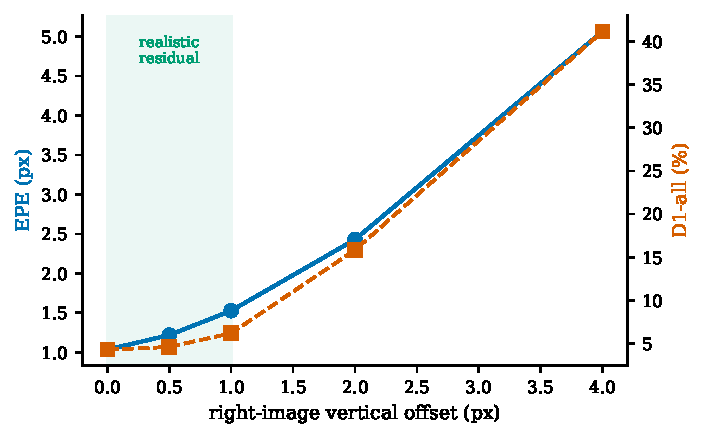
\includegraphics[width=0.85\columnwidth]{fig_4_9_rectification}
\caption{\textbf{End-point error and D1-all against vertical rectification offset.} Degradation is graceful up to one pixel and steep beyond.}
\label{fig:rect}
\end{figure}

\subsection{Real-Rig Agreement}
To confirm this tolerance on physical data, we ran the checkpoint on 997 rectified pairs from a low-cost 52 mm baseline stereo rig (AR0144 sensors, focal length approximately 1005 px at the native 1280 px width) whose factory rectification leaves residual vertical misalignment, and compared it against FoundationStereo \cite{wen2025foundationstereo} pseudo-ground-truth on the same pairs. Mean EPE is 1.45 px and D1-all is 11.1 percent. Since both models see the same imperfect input, this figure measures agreement with a strong reference rather than absolute error; it corroborates, but does not replace, the controlled sweep.

\subsection{Deployment and Latency}
Reaching the embedded latency target required optimizing the inference graph, not just training the network. Six changes, each proven equivalent bitwise or through a matched A/B comparison, cut full-precision latency on the RTX 3050 from 106.7 to 61.4 ms, a 1.74$\times$ speedup: zero-copy padded views in the cost-volume loops, batched correlation lookups with cached sampling grids, hoisting the static recurrent-input channels to run once per scale, fusing the gate convolutions and output heads, removing dead inference-path code, and narrowing the geometry volume to its $\pm 16$ band. Three further operator swaps cleared the blocks to eight-bit deployment (the unfold in convex upsampling, group normalization, and 3D convolution on some toolchains), after which the graph was exported and calibrated to an INT8 TensorRT engine. Table \ref{tab:latency} reports the measured result: 36.3 ms per frame, or 27.5 FPS, on the Jetson Orin Nano within roughly 0.15 GB, near the 30 FPS real-time target on the intended device rather than a desktop proxy.

\begin{table}[!htbp]
\centering
\caption{\textbf{Measured latency and memory at batch 1, $384\times 640$} (10 warm-up, 100 timed passes; Jetson memory is estimated).}
\label{tab:latency}
\footnotesize
\setlength{\tabcolsep}{3.4pt}
\begin{tabular}{lccc}
\toprule
Configuration & Latency (ms) & FPS & Memory (GB)\\
\midrule
RTX 3050 laptop, fp32 & 61.4 & 16.3 & 0.35\\
RTX 3050 laptop, fp16 & 49.8 & 20.1 & 0.26\\
Orin Nano, INT8 TensorRT & 36.3 & 27.5 & ${\sim}0.15$\\
\bottomrule
\end{tabular}
\end{table}

\subsection{Ablation Studies}
Table \ref{tab:ablations} summarizes the four controlled studies behind the production configuration; each varied a single factor on a matched harness. The training recipe, not any architectural block, was the largest single accuracy lever: the augmentation triplet lowered the best validation EPE from 2.778 to 1.921 px in a matched comparison, a 31 percent reduction. The inference-efficiency pass held accuracy while cutting harness latency from 46.6 to 30.2 ms, with EPE unchanged within noise (2.908 to 2.906 px); the narrow geometry band, the only accuracy-relevant change in the pass, was validated separately as neutral. In the boundary-sharpness study, plane rendering cut the bad-0.5 rate from 55.36 to 42.91 percent and was also the fastest variant; composing it with a bimodal head or top-k initialization worsened results (44.40 and 46.58 percent), so we adopted plane rendering alone. The input-protocol study showed that training on native-resolution crops cut the native-axis EPE from 6.672 to 2.869 px versus the legacy global-resize protocol (2.967 for native full frames), at no cost on the resized axis (1.783 px for both), and the native-crop protocol was adopted for the production run. Earlier campaigns on a smaller tile chassis selected the remaining components: the YOLO26s encoder over GhostConv and YOLO26n, iterated coarse-to-fine refinement over single-pass propagation (which collapsed EPE from 0.578 to 0.844 px), and the threshold-stack-plus-D1 objective over eight alternatives.

\begin{table}[!htbp]
\centering
\caption{\textbf{Controlled ablation summary.} Each study varies one factor on a matched harness; metrics differ per study and are stated per row.}
\label{tab:ablations}
\footnotesize
\setlength{\tabcolsep}{4pt}
\begin{tabular}{llcc}
\toprule
Study & Metric & Baseline & Adopted\\
\midrule
Augmentation triplet & val EPE (px) & 2.778 & \textbf{1.921}\\
Efficiency pass & latency (ms) / EPE & 46.6 / 2.908 & \textbf{30.2} / 2.906\\
Plane rendering & bad-0.5 (\%) & 55.36 & \textbf{42.91}\\
Native-crop input & native-axis EPE (px) & 6.672 & \textbf{2.869}\\
\bottomrule
\end{tabular}
\end{table}

\section{Limitations}
\label{sec:limits}
Several limits bound these conclusions. First, all zero-shot numbers are computed on public training splits under our own protocol; the model has not been submitted to any official leaderboard, and the 192 px disparity cap of our protocol removes the largest disparities of Middlebury 2014. Second, a clear gap remains to the distillation-trained and iterative references on Middlebury, concentrated in scenes with dense thin repeated structures and near-cap disparities, exactly where quarter-resolution reasoning with a bounded search performs worst; the convex upsampler can recombine coarse disparities but cannot invent hypotheses absent at 1/4 resolution. Third, rectification tolerance holds only across the sub-pixel to one-pixel range that a calibrated rig produces; beyond two pixels of vertical offset, accuracy collapses. Fourth, the real-rig figure measures agreement with a FoundationStereo reference, not absolute error against ground truth. Finally, the results come from a single training run, so run-to-run variance is unknown, and the model performs no explicit occlusion reasoning or left-right consistency checking.

\section{Conclusion}
\label{sec:conclusion}
We presented StereoLite, a 2.96 M parameter stereo network that composes a slanted tile-plane state, recurrent GRU refinement with local correlation, a narrow-band geometry encoding volume with learned fail-soft fusion, and plane rendering with convex upsampling, all inside an INT8-clean operator set. Trained on SceneFlow alone, a single checkpoint reaches 4.33, 3.93, 3.96, and 10.9 percent D1-all zero-shot on KITTI 2012, KITTI 2015, ETH3D, and Middlebury 2014 under one fixed protocol, runs at 36.3 ms per frame on a Jetson Orin Nano after graph optimization and TensorRT calibration, and tolerates up to one pixel of vertical rectification error. The remaining gap to larger distillation-trained models is localized to an identifiable scene type rather than diffuse, which makes knowledge distillation from foundation-scale teachers the natural next step for closing it at this parameter budget.

\bibliographystyle{IEEEtran}
\bibliography{refs}

\end{document}
